\documentclass[acmtog]{acmart}
\usepackage{graphicx}
\usepackage{subfigure}
\usepackage{natbib}
\usepackage{listings}
\usepackage{bm}
\usepackage{graphicx}
\usepackage{subfigure}

\definecolor{blve}{rgb}{0.3372549 , 0.61176471, 0.83921569}
\definecolor{gr33n}{rgb}{0.29019608, 0.7372549, 0.64705882}
\makeatletter
\lst@InstallKeywords k{class}{classstyle}\slshape{classstyle}{}ld
\makeatother
\lstset{language=C++,
	basicstyle=\ttfamily,
	keywordstyle=\color{blve}\ttfamily,
	stringstyle=\color{red}\ttfamily,
	commentstyle=\color{magenta}\ttfamily,
	morecomment=[l][\color{magenta}]{\#},
	classstyle = \bfseries\color{gr33n}, 
	tabsize=2
}
\lstset{basicstyle=\ttfamily}

% Title portion
\title{Warm-up assignment:\\ {Programming simple graphics program with OpenGL}} 

\author{Name:\quad Xiaohan Wu  \\ student number:\ 2019533093
\\email:\quad wuxh@shanghaitech.edu.cn}

% Document starts
\begin{document}
\maketitle

\vspace*{2 ex}

\section{Introduction}
This is a warm up assignment for CS171.01.To finish this homework, we can use either immediate mode or core mode to realize what we have in mind. For me, I try to use core mode to draw a rectangle using opengl.
\section{Implementation Details}
First,we have to create two necessary shaders:vertex shader and fragment shader, and link them together to create a shader program. As I want to realize the gradient color of the rectangular, I have to pass the color information from vertex shader to the fragment shader, and during the pass, opengl will automatically interpolate the residual color inside the triangle.
After that, we create VAO and VBO and vertex attribute pointer corresponding to how we pass the information of predetermined data to the vertex shader.
Finally, we get what we want to draw: a rectangular with gradient color.  
\section{Results}
Here is the result of my work.
\begin{figure}[h]
	\centering
	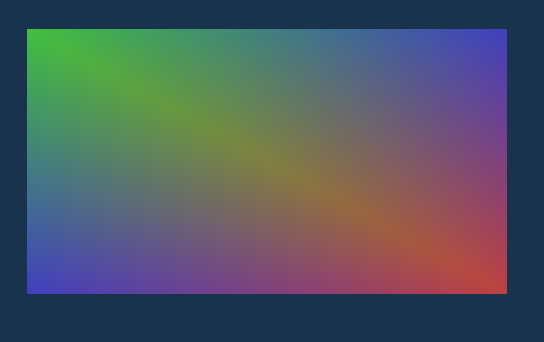
\includegraphics[width=4cm,height=5cm]{show.PNG}
	\caption{Rectangular}
\end{figure}

\end{document}
